\chapter{System Analysis}

\setlength{\parindent}{1em}

\section{Introduction}

This chapter analyzes MiPay as a system: what it must do, the constraints it
operates under, and the models that describe its structure and behavior. The
analysis follows standard software-engineering practice---requirements
specification followed by a sequence of complementary diagrams (context,
data-flow, entity-relationship, use-case, class, activity, and sequence)---but
each model is specialized to MiPay's defining characteristic: a stateless,
human-in-the-loop AI pipeline that converts bilingual speech into validated
financial records. The diagrams referenced throughout this chapter are provided
as figures; the corresponding source artwork is catalogued in the figure guide
that accompanies this document.

\section{System Requirements}

Requirements are divided into functional requirements (FRs), which specify what
the system does, and non-functional requirements (NFRs), which specify quality
attributes and constraints.

\subsection{Functional Requirements}

\begin{longtable}{>{\bfseries}p{1.6cm} p{12.5cm}}
\caption{Functional requirements.}\label{tab:fr}\\
\toprule
\textbf{ID} & \textbf{Requirement} \\
\midrule
\endfirsthead
\toprule
\textbf{ID} & \textbf{Requirement} \\
\midrule
\endhead
\bottomrule
\endfoot
FR-01 & A user can register with email and password and log in; sessions persist via refresh tokens. \\
FR-02 & A user can record a voice note (maximum 30 seconds) from the home screen with a single tap to start and a tap to stop. \\
FR-03 & The recorded audio is uploaded to the backend, which returns the transcript \emph{and} the extracted transaction fields in one response. \\
FR-04 & Extraction must work for Modern Standard Arabic, common Arabic dialects (Gulf, Egyptian, Levantine---best effort), English, and mixed Arabic--English code-switching. \\
FR-05 & The extracted fields are type (expense/income), amount, currency, category, name, and date; missing fields are returned as null, except type and amount which are required (see FR-07). \\
FR-06 & Relative dates (``yesterday'', dialectal ``\emph{ams}'', ``last Friday'', ``\emph{qabl yomayn}'') are resolved to absolute ISO dates server-side using the device-supplied current date. \\
FR-07 & If amount cannot be extracted, the API returns a structured ``needs\_review'' result and the app opens a manual form pre-filled with whatever was extracted. \\
FR-08 & Before saving, the app shows a confirmation step where the user can edit any field; categories are chosen from a fixed bilingual list. \\
FR-09 & A user can create, view, edit, and delete transactions manually (full CRUD). \\
FR-10 & A user can view transactions in a list, filterable by month, category, and type, sorted newest-first. \\
FR-11 & A user can view a monthly dashboard: total income, total expense, net balance, and an expenses-per-category breakdown. \\
FR-12 & The UI is fully localized in Arabic (RTL) and English (LTR); the user can switch language in settings; the default follows the device locale. \\
FR-13 & Users can only ever access their own data, enforced server-side on every endpoint. \\
FR-14 & A user can add a transaction by \emph{typing} a natural-language sentence (text mode), which runs the same extraction pipeline without the speech stage. \\
FR-15 & A single utterance describing several transactions yields several editable records, savable atomically in one operation. \\
\end{longtable}

\subsection{Non-Functional Requirements}

\begin{longtable}{>{\bfseries}p{1.7cm} p{12.4cm}}
\caption{Non-functional requirements.}\label{tab:nfr}\\
\toprule
\textbf{ID} & \textbf{Requirement} \\
\midrule
\endfirsthead
\toprule
\textbf{ID} & \textbf{Requirement} \\
\midrule
\endhead
\bottomrule
\endfoot
NFR-01 & End-to-end voice latency target: $\leq$\,10\,s for a 10-second clip on the CPU-only reference server; $\leq$\,4\,s with a GPU. A progress indicator is shown during processing. \\
NFR-02 & Extraction quality targets on the evaluation set: $\geq$\,90\% exact-match on amount, $\geq$\,85\% on type, $\geq$\,80\% on category; STT targets WER $\leq$\,20\% (Arabic), $\leq$\,12\% (English). \\
NFR-03 & Passwords hashed with bcrypt; JWTs signed with HS256; secrets supplied only through environment variables; HTTPS assumed at the reverse-proxy layer. \\
NFR-04 & Audio files are deleted from the server immediately after processing; only the transcript is retained, attached to its transaction for traceability. \\
NFR-05 & All API responses use a consistent JSON envelope and a uniform error format. \\
NFR-06 & The backend runs on a single machine with 16\,GB RAM and no GPU (GPU is optional acceleration). \\
NFR-07 & Backend code is typed and unit-tested (post-processing and auth in particular); the Flutter client is analyzer-clean. \\
NFR-08 & The entire system is reproducible via Docker Compose; a documented one-command setup brings up all services. \\
\end{longtable}

\section{Context Diagram}

The context diagram (Figure~\ref{fig:context}) frames MiPay as a single process
interacting with one external actor---the authenticated user---and three
internal supporting subsystems that, from the user's standpoint, are
encapsulated: the speech-to-text engine, the language-model extraction server,
and the relational datastore. Unlike a typical cloud application, MiPay has
\emph{no} external third-party data flows: no audio or text leaves the operator's
deployment boundary. This absence of outward arrows is itself a design statement
and is what grounds the project's privacy and zero-cost claims.

\begin{figure}[H]
    \centering
    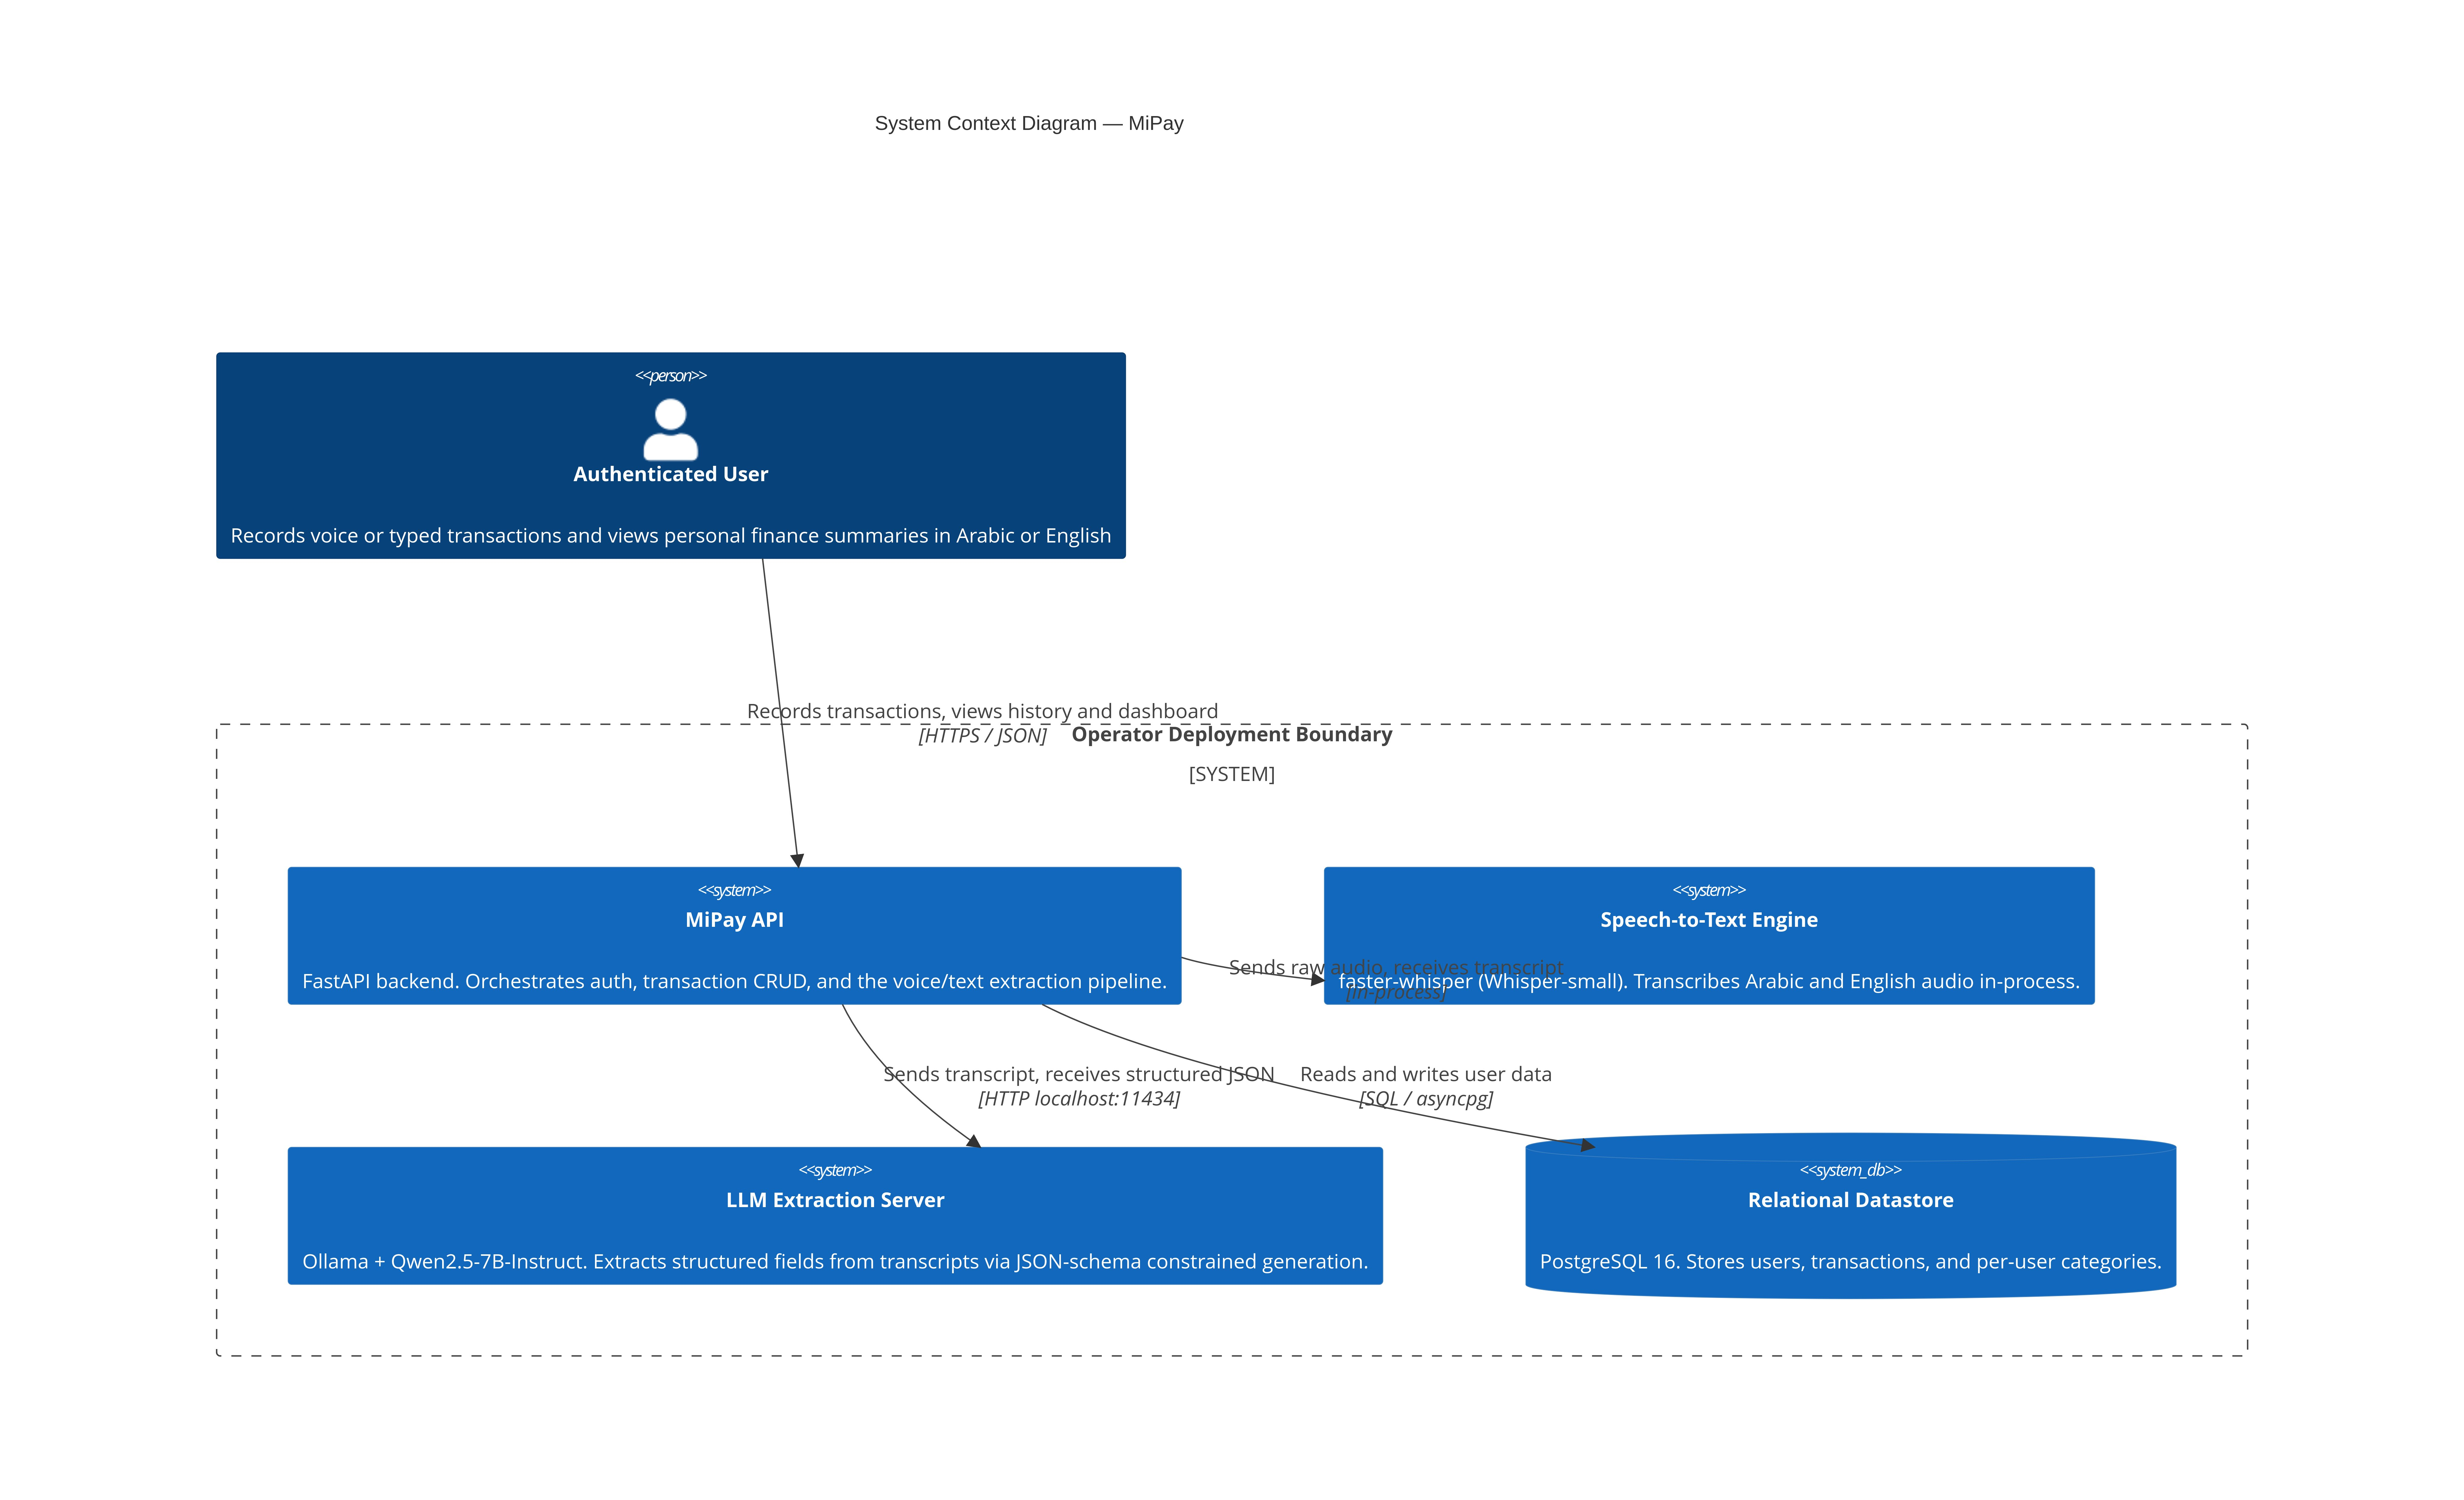
\includegraphics[width=0.75\textwidth]{figures/context_diagram.jpg}
    \caption[System context diagram]{System context diagram. The user is the only
    external actor; the speech engine, the LLM extraction server, and the
    database are internal subsystems within the deployment boundary. No data
    crosses the boundary to any third party.}
    \label{fig:context}
\end{figure}

\section{Data Flow Diagram (DFD)}

The data-flow view decomposes the system into the transformations a request
undergoes. Figure~\ref{fig:dfd0} shows the level-0 (context-level) DFD, and
Figure~\ref{fig:dfd1} expands the voice-processing process into its constituent
sub-processes: audio normalization, transcription, numeral normalization,
constrained extraction, and deterministic post-processing.

\begin{figure}[H]
    \centering
    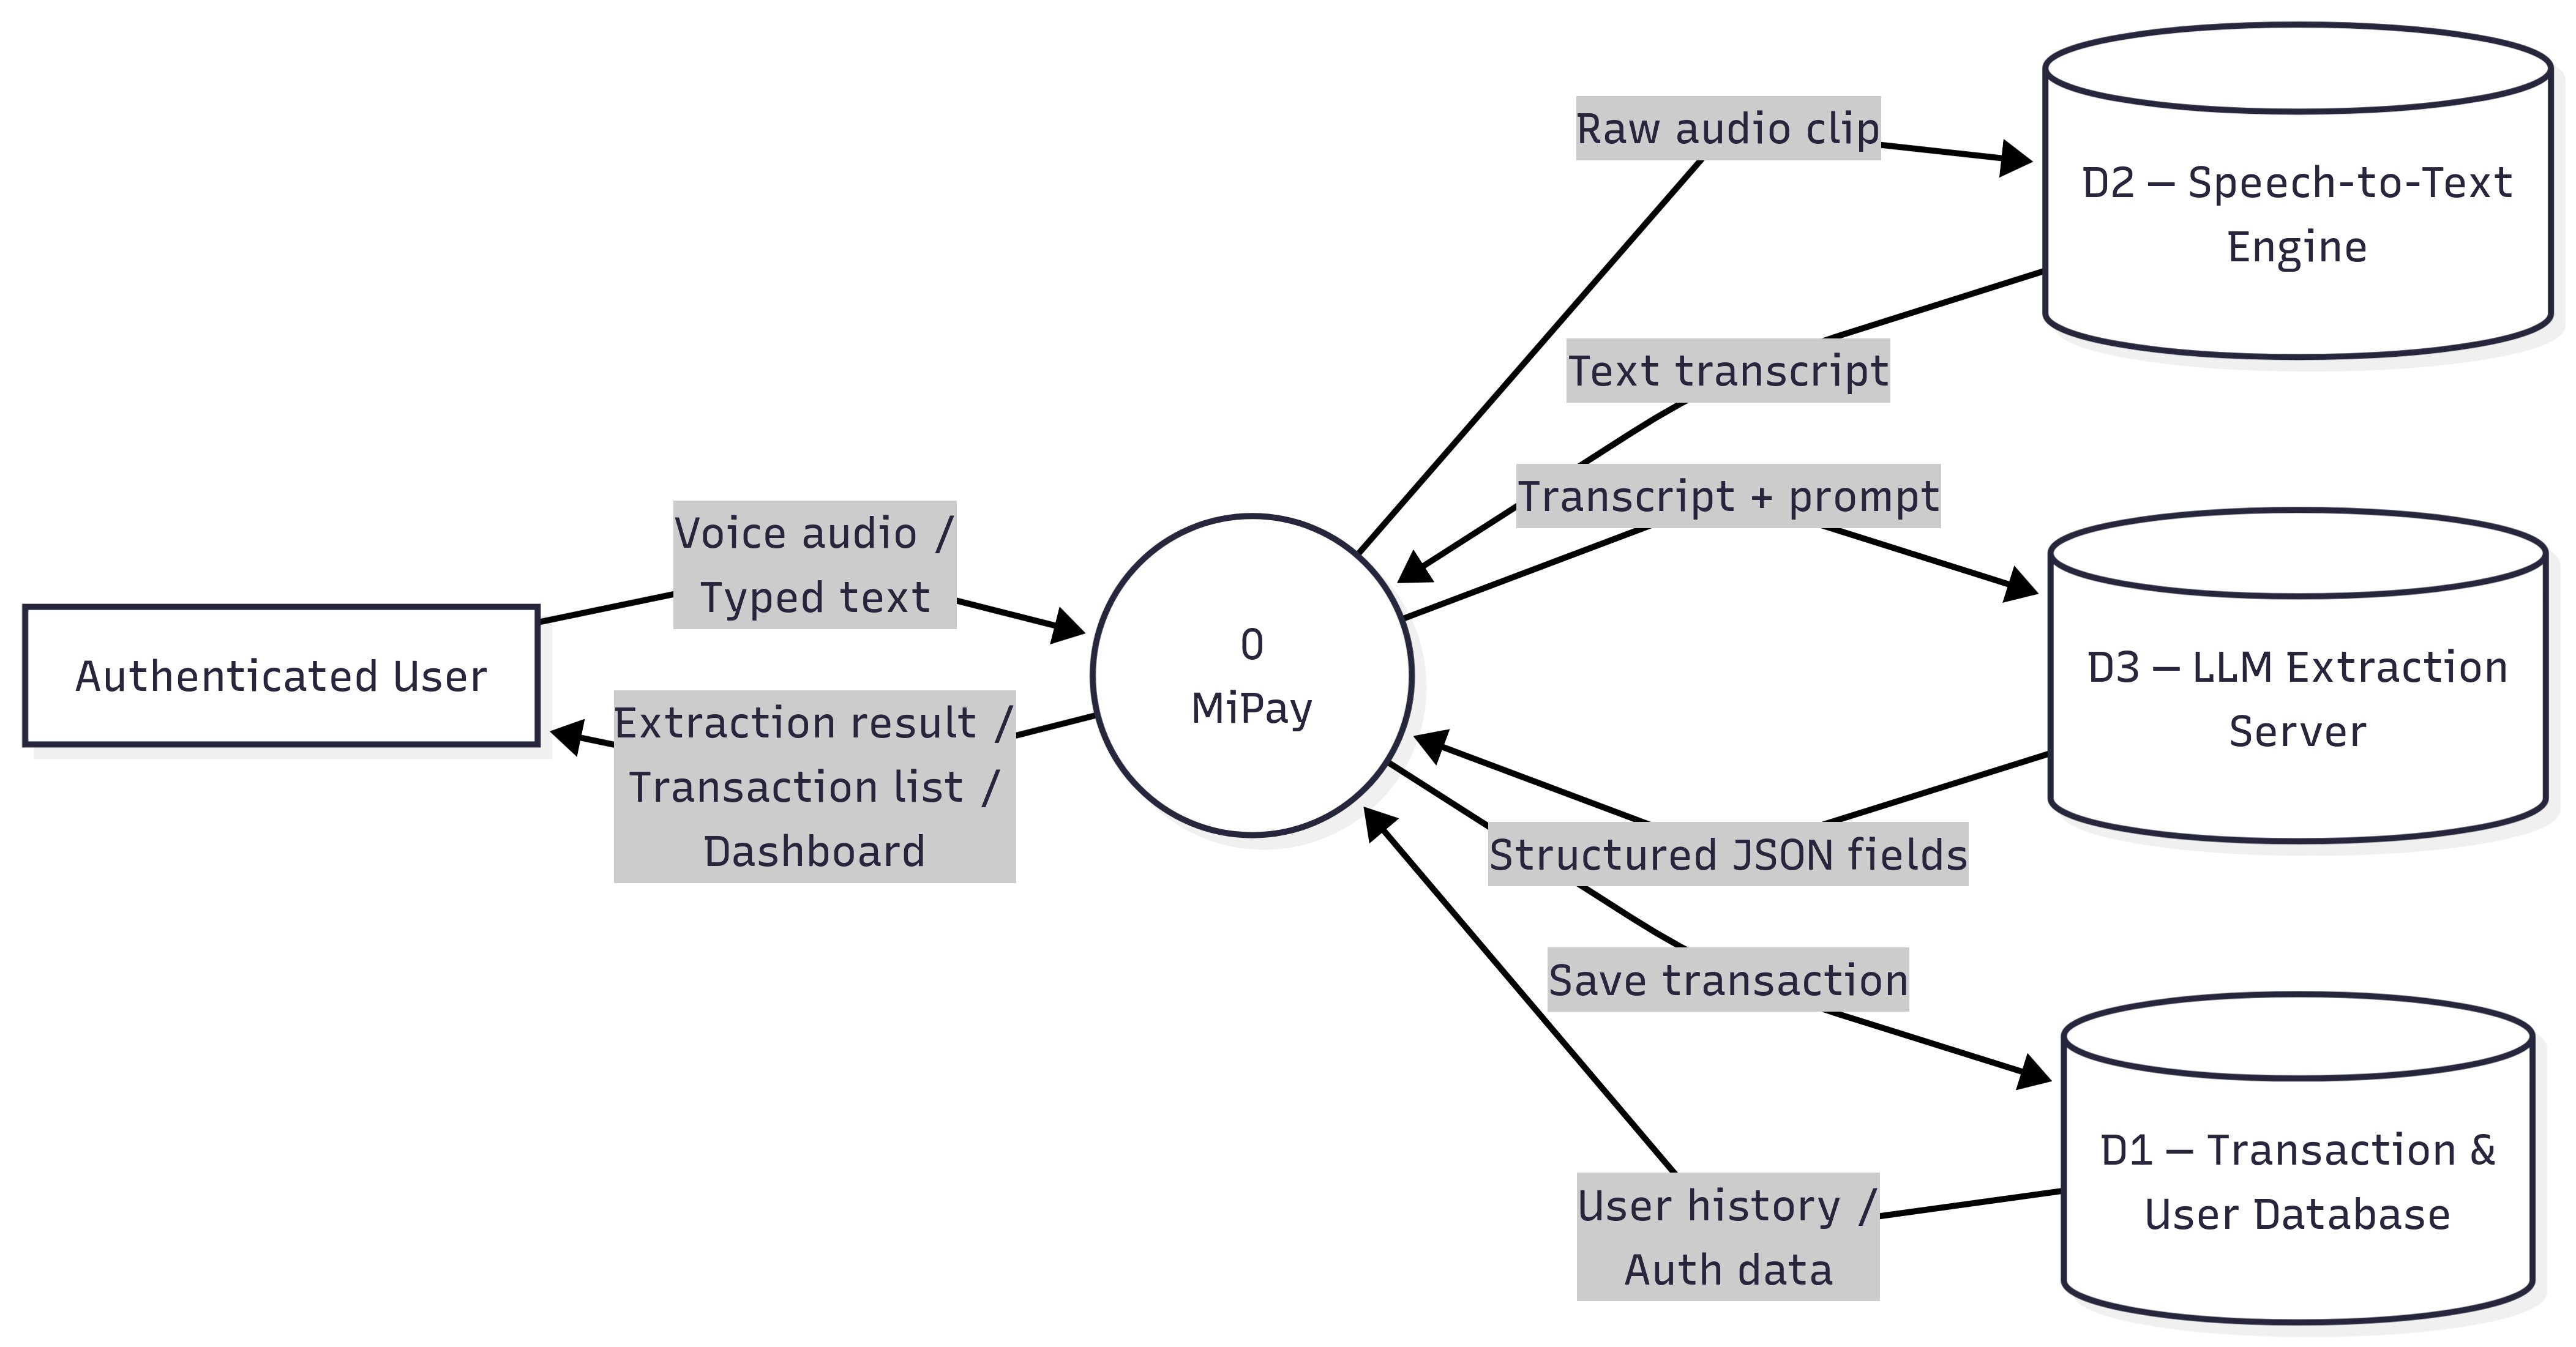
\includegraphics[width=0.8\textwidth]{figures/dfd_level0.jpg}
    \caption[Level-0 data-flow diagram]{Level-0 data-flow diagram. A voice or text
    request flows into the MiPay process, which consults the speech and language
    subsystems and the transaction store, and returns a structured extraction
    result.}
    \label{fig:dfd0}
\end{figure}

\begin{figure}[H]
    \centering
    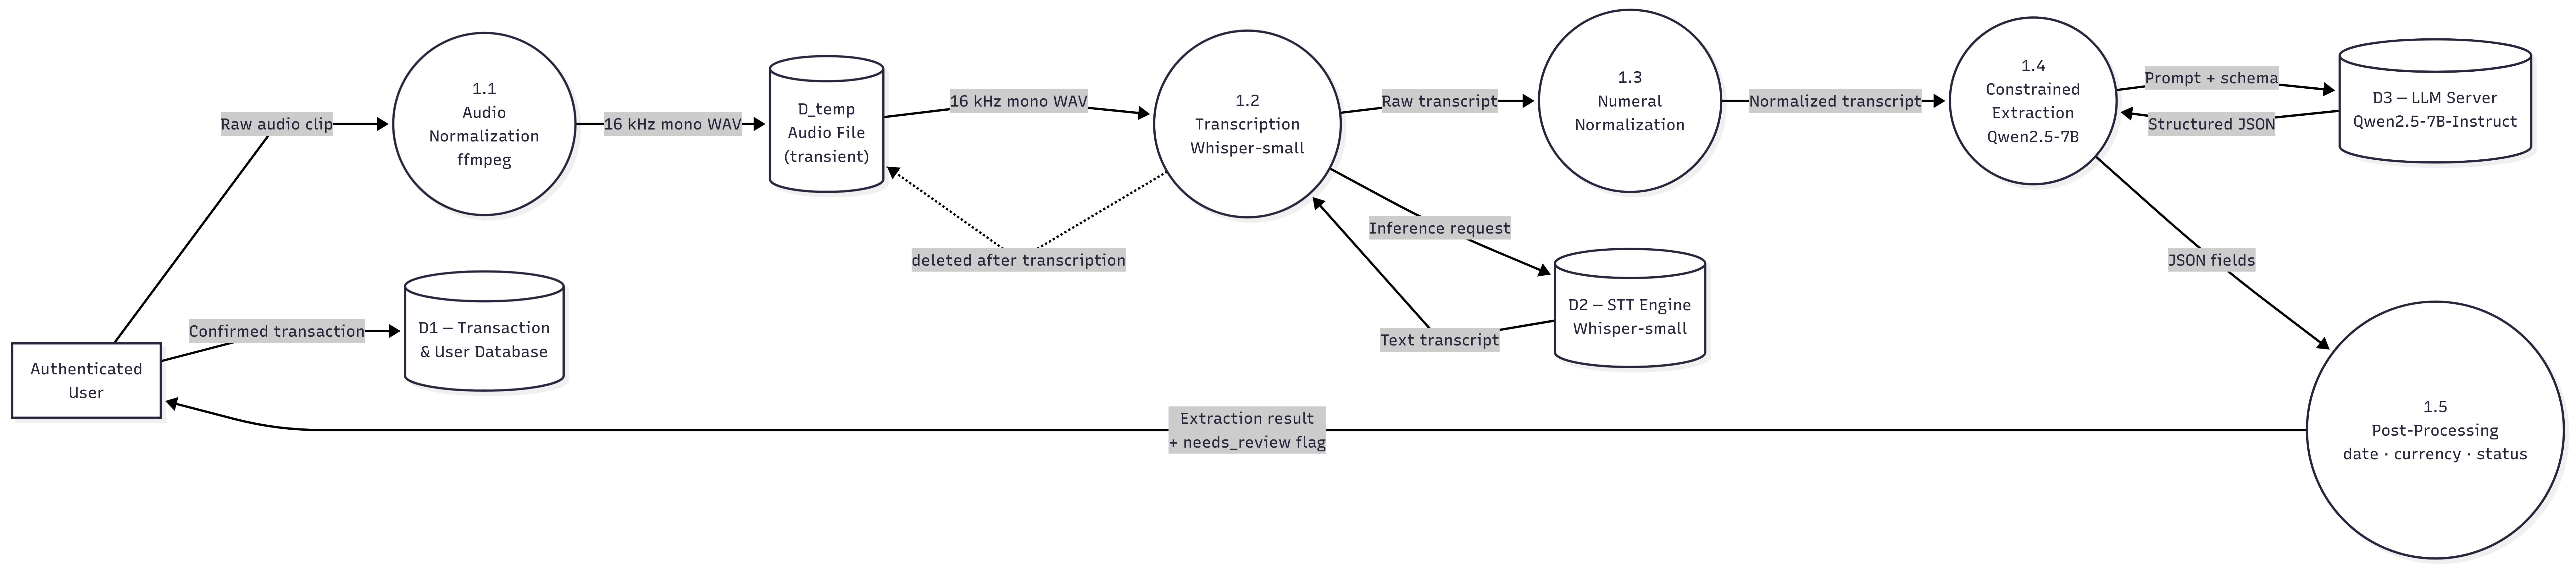
\includegraphics[width=\textwidth]{figures/dfd_level1.jpg}
    \caption[Level-1 data-flow diagram of the voice pipeline]{Level-1 data-flow
    diagram of the voice pipeline. Audio is converted to 16\,kHz mono WAV,
    transcribed by Whisper, numeral-normalized, sent to the constrained LLM
    extractor, and finally passed through the deterministic post-processing layer
    (date resolution, currency defaulting, status decision) before the response is
    assembled. Audio is deleted immediately after transcription.}
    \label{fig:dfd1}
\end{figure}

A defining property visible in the DFD is that the voice-processing data store
for audio is \emph{transient}: the audio file exists only between upload and
transcription and is deleted thereafter (NFR-04). The only persistent store is
the transaction/user database, written exclusively by the explicit
save operation that follows user confirmation---never by the AI pipeline itself.

\section{Entity-Relationship (ER) Diagram}

The persistent data model comprises three entities: \texttt{users},
\texttt{transactions}, and a seed \texttt{categories} table.
Figure~\ref{fig:erd} shows their relationships. A user owns many transactions
(one-to-many, cascade on delete); every transaction references exactly one
category by key (many-to-one against the seed table). The category table is fixed
reference data---seeded once via migration---holding the bilingual labels and an
icon name for each of the twenty-nine categories.

\begin{figure}[H]
    \centering
    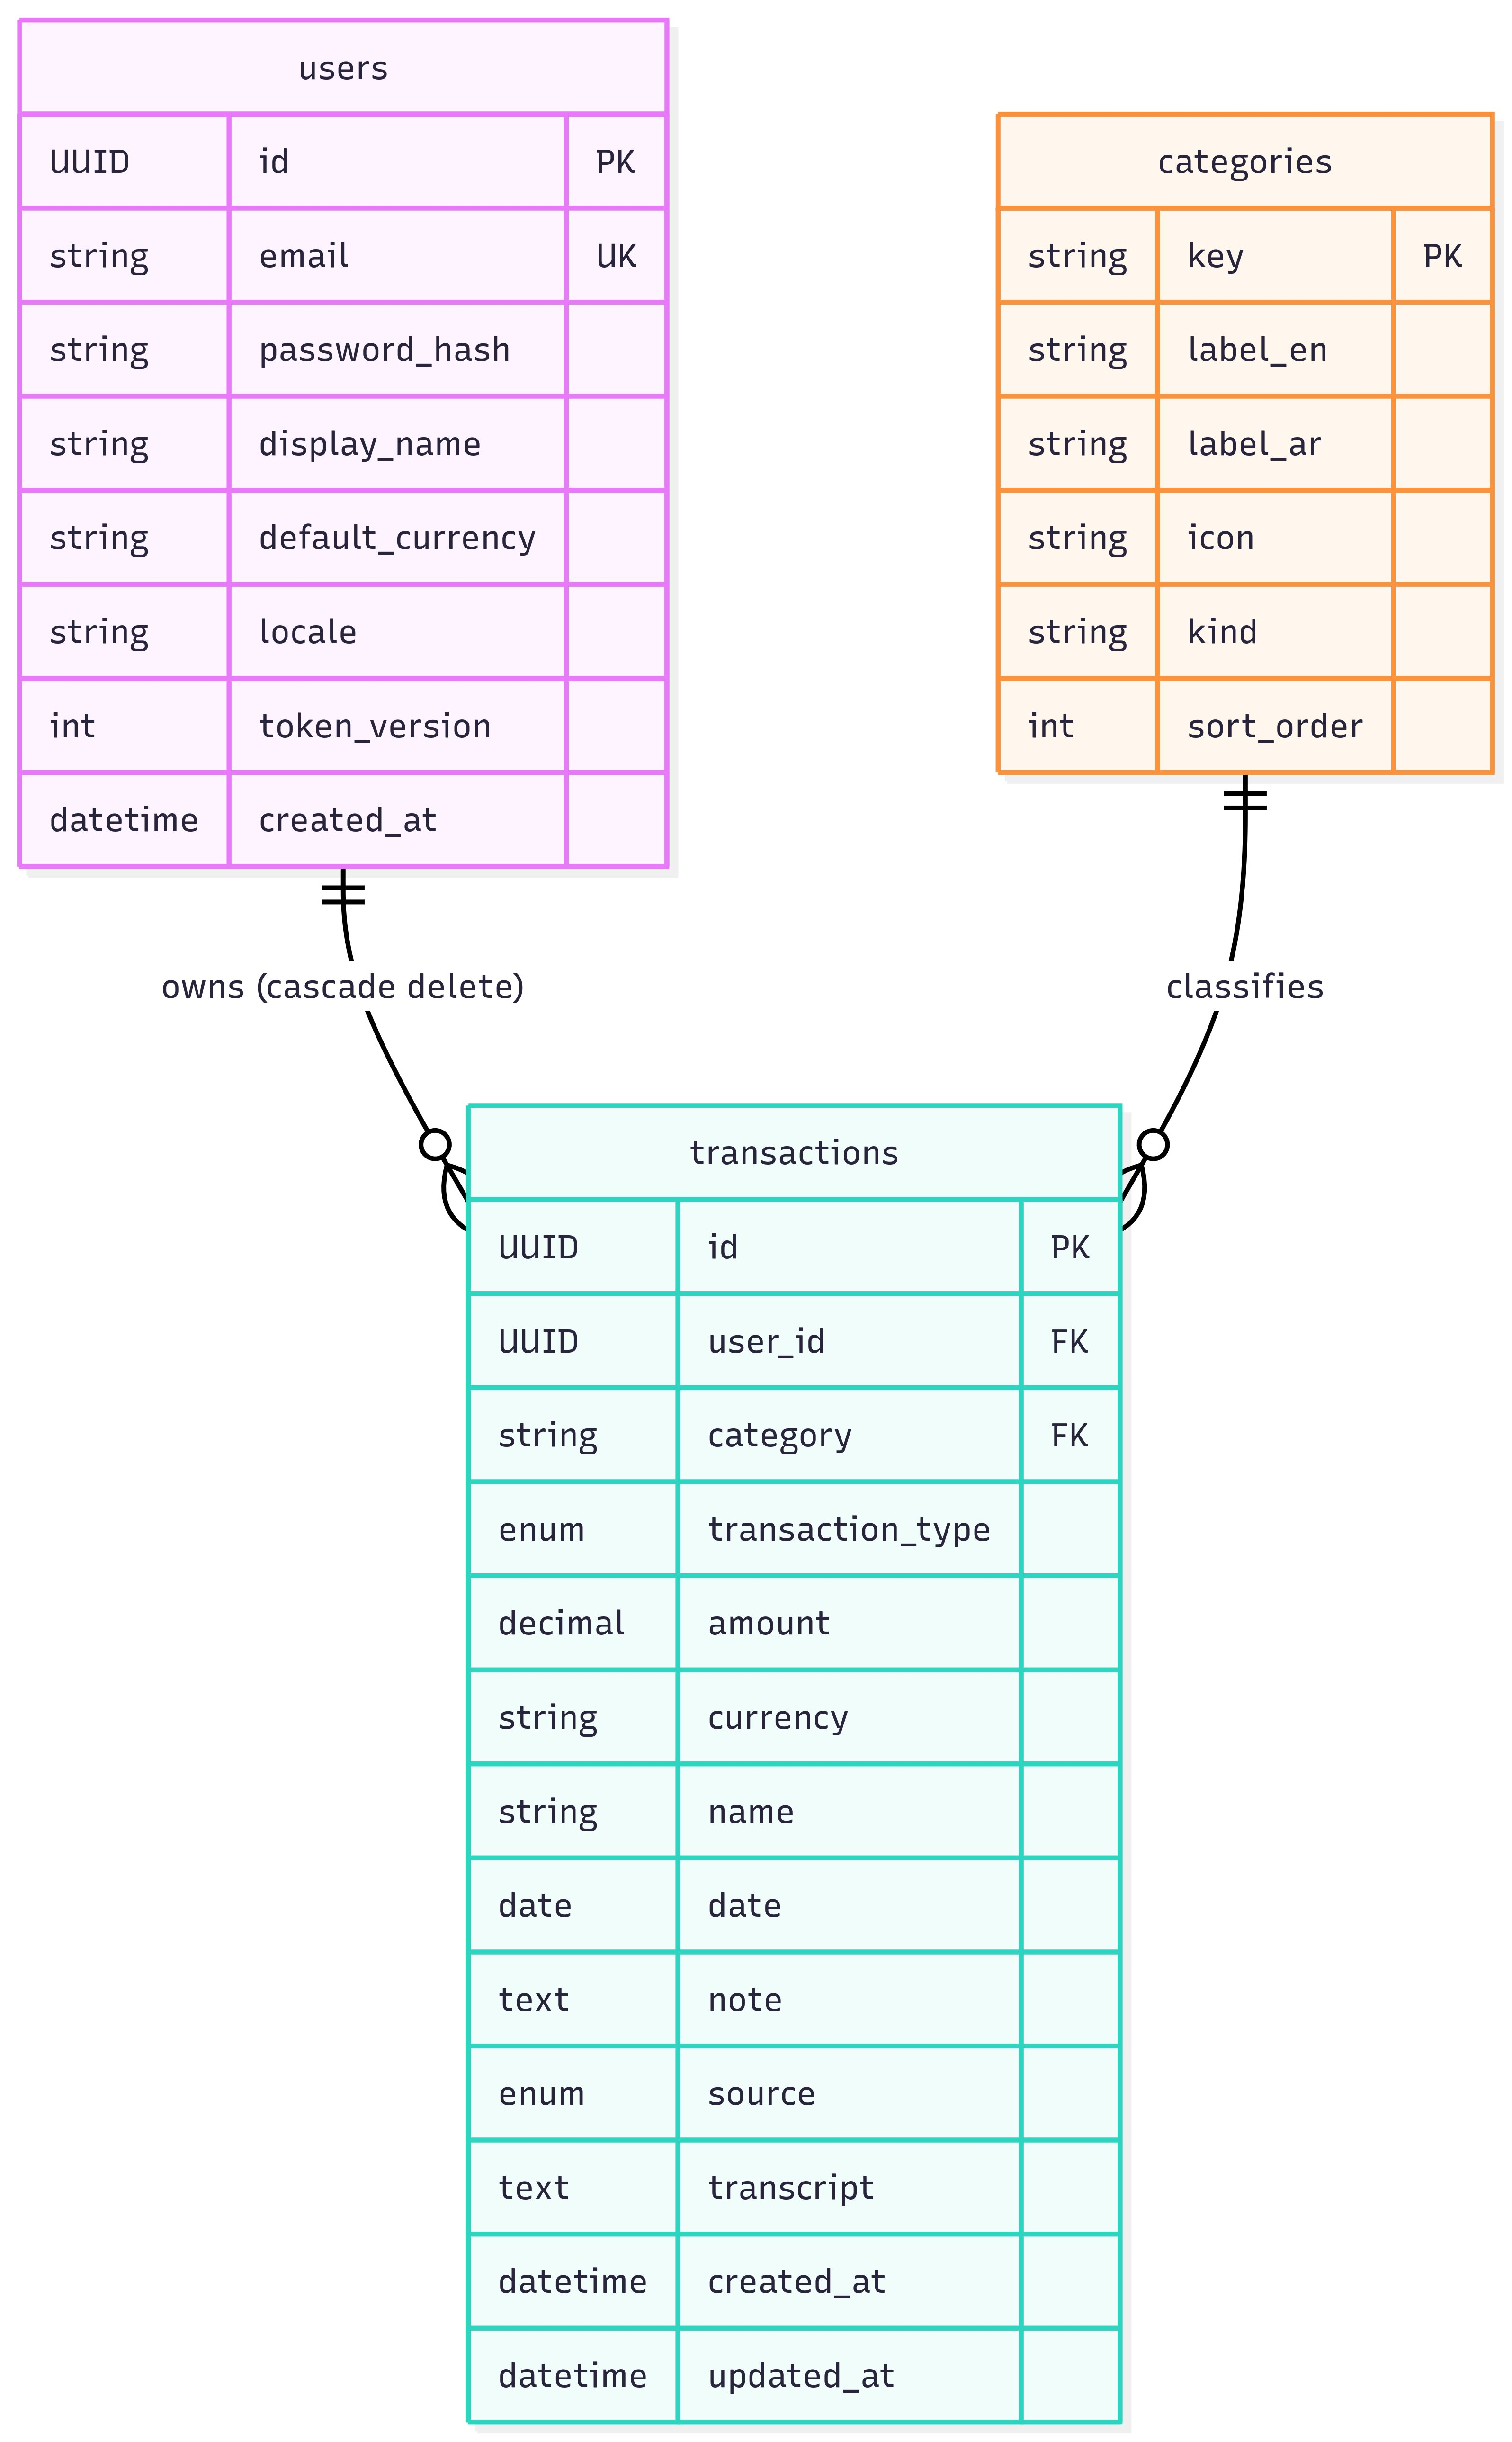
\includegraphics[width=0.85\textwidth]{figures/er_diagram.jpg}
    \caption[Entity-relationship diagram]{Entity-relationship diagram. A
    \texttt{user} has many \texttt{transactions}; each \texttt{transaction}
    references one \texttt{category} from the seeded bilingual category table.
    Deleting a user cascades to their transactions.}
    \label{fig:erd}
\end{figure}

\subsection{Mapping}

The conceptual ER model maps to the relational schema in
Table~\ref{tab:schema-map}. Monetary amounts are stored as fixed-point
\texttt{NUMERIC(12,2)} rather than floating point to avoid representation error,
and two PostgreSQL enumerated types constrain \texttt{transaction\_type} and
\texttt{source}. Two composite indexes---\texttt{(user\_id, date DESC)} and
\texttt{(user\_id, category)}---support the list and summary queries, which are
always scoped to a single user.

\begin{table}[H]
\centering
\caption{Mapping of entities to relational tables (principal columns).}
\label{tab:schema-map}
\small
\renewcommand{\arraystretch}{1.25}
\begin{tabularx}{\textwidth}{l l X}
\toprule
\textbf{Table} & \textbf{Key columns} & \textbf{Notes} \\
\midrule
\texttt{users} & \texttt{id} (UUID PK), \texttt{email} (unique) & \texttt{password\_hash}, \texttt{display\_name}, \texttt{default\_currency}, \texttt{locale}, \texttt{token\_version}, \texttt{created\_at}. \\
\texttt{transactions} & \texttt{id} (UUID PK), \texttt{user\_id} (FK) & \texttt{transaction\_type} (enum), \texttt{amount} \texttt{NUMERIC(12,2)}, \texttt{currency}, \texttt{category} (FK), \texttt{name}, \texttt{date}, \texttt{note}, \texttt{source} (enum), \texttt{transcript}, timestamps. \\
\texttt{categories} & \texttt{key} (PK) & \texttt{label\_en}, \texttt{label\_ar}, \texttt{icon}, \texttt{kind} (expense/income/both), \texttt{sort\_order}; seeded reference data. \\
\bottomrule
\end{tabularx}
\end{table}

\section{Use Case Diagrams}

Figure~\ref{fig:usecase} presents the use-case model. The single actor,
\emph{Authenticated User}, drives all use cases; an internal \emph{AI Pipeline}
actor is shown to clarify which use cases are served by the speech and language
subsystems. The principal use cases are: register/login, record voice
transaction, type text transaction, enter transaction manually, confirm/edit
extracted transactions, list and filter transactions, edit/delete a transaction,
view the monthly dashboard, and change settings (language and default currency).

\begin{figure}[H]
    \centering
    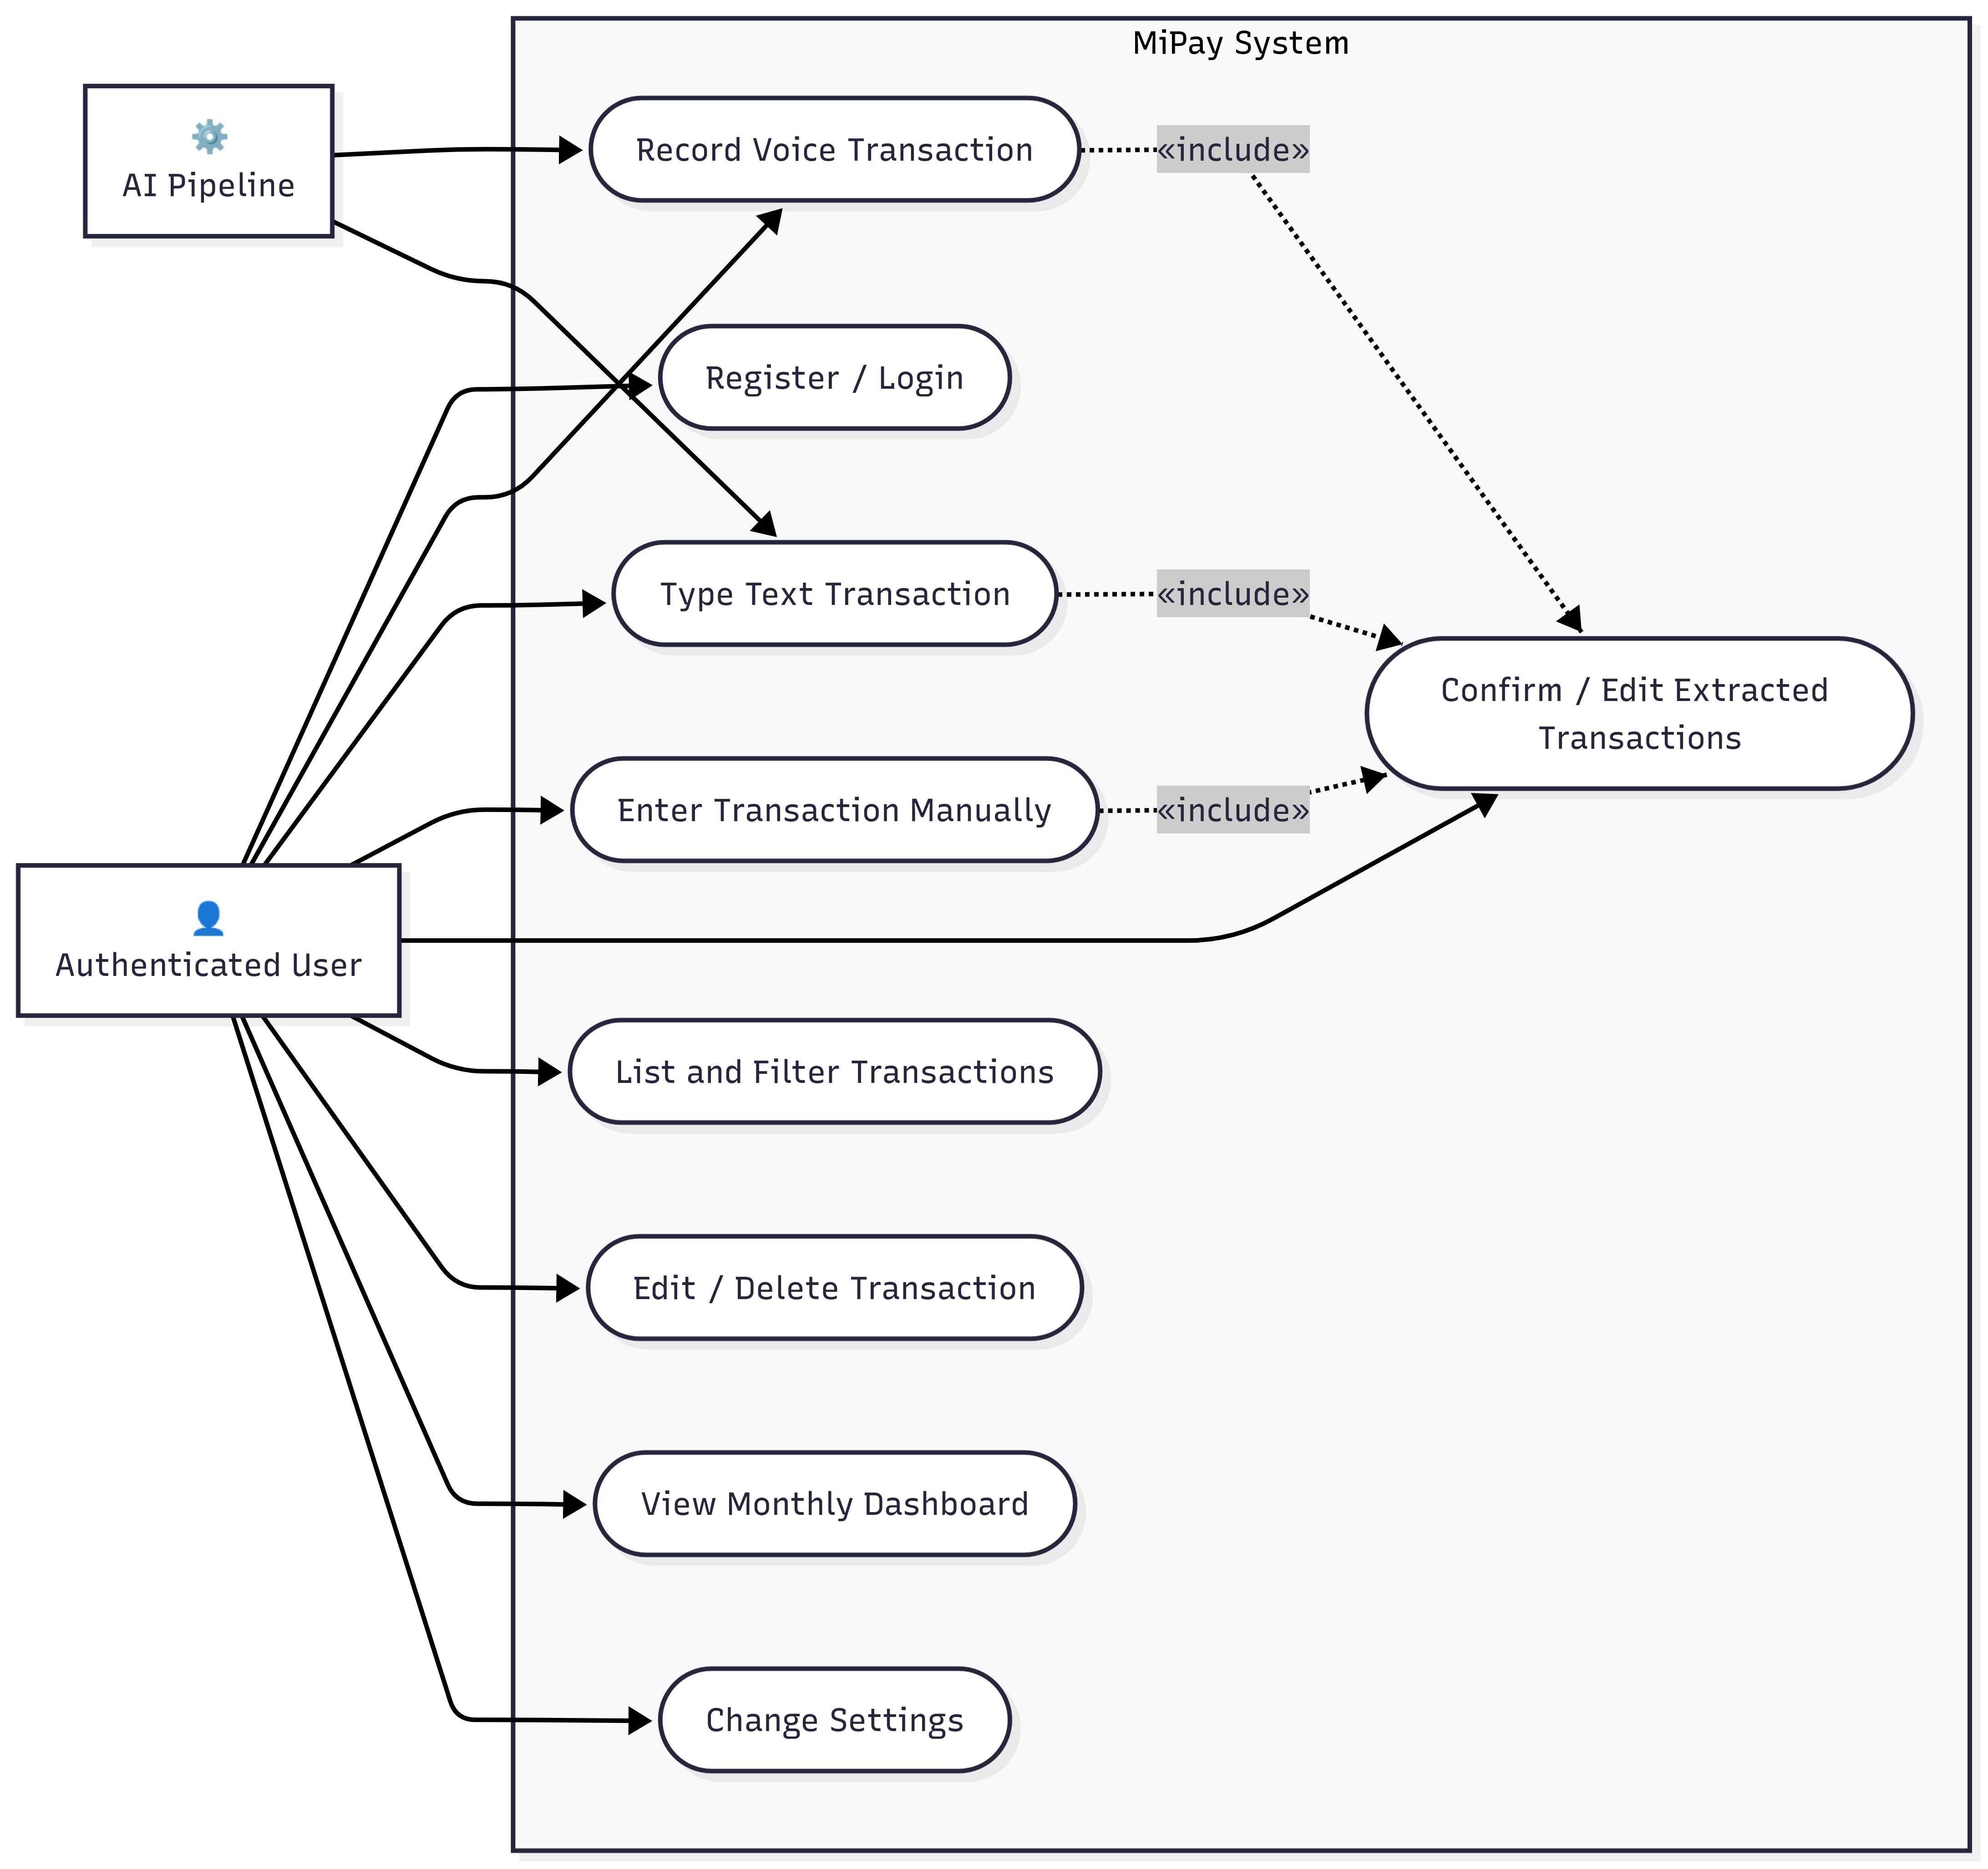
\includegraphics[width=0.9\textwidth]{figures/use_case_diagram.jpg}
    \caption[Use-case diagram]{Use-case diagram. The authenticated user drives all
    use cases. The three input modes (voice, text, manual) all
    \texttt{<<include>>} the shared confirm-and-save use case; the AI pipeline
    serves the voice and text extraction use cases.}
    \label{fig:usecase}
\end{figure}

\section{Activity Diagrams}

The activity diagram in Figure~\ref{fig:activity-voice} models the control flow
of the central voice use case, including the decision points that route an
utterance to \texttt{ok}, \texttt{needs\_review}, or \texttt{failed} outcomes.
The flow makes explicit that no database write occurs until after the user
confirms; the AI pipeline only \emph{proposes}.

\begin{figure}[p]



    \centering
   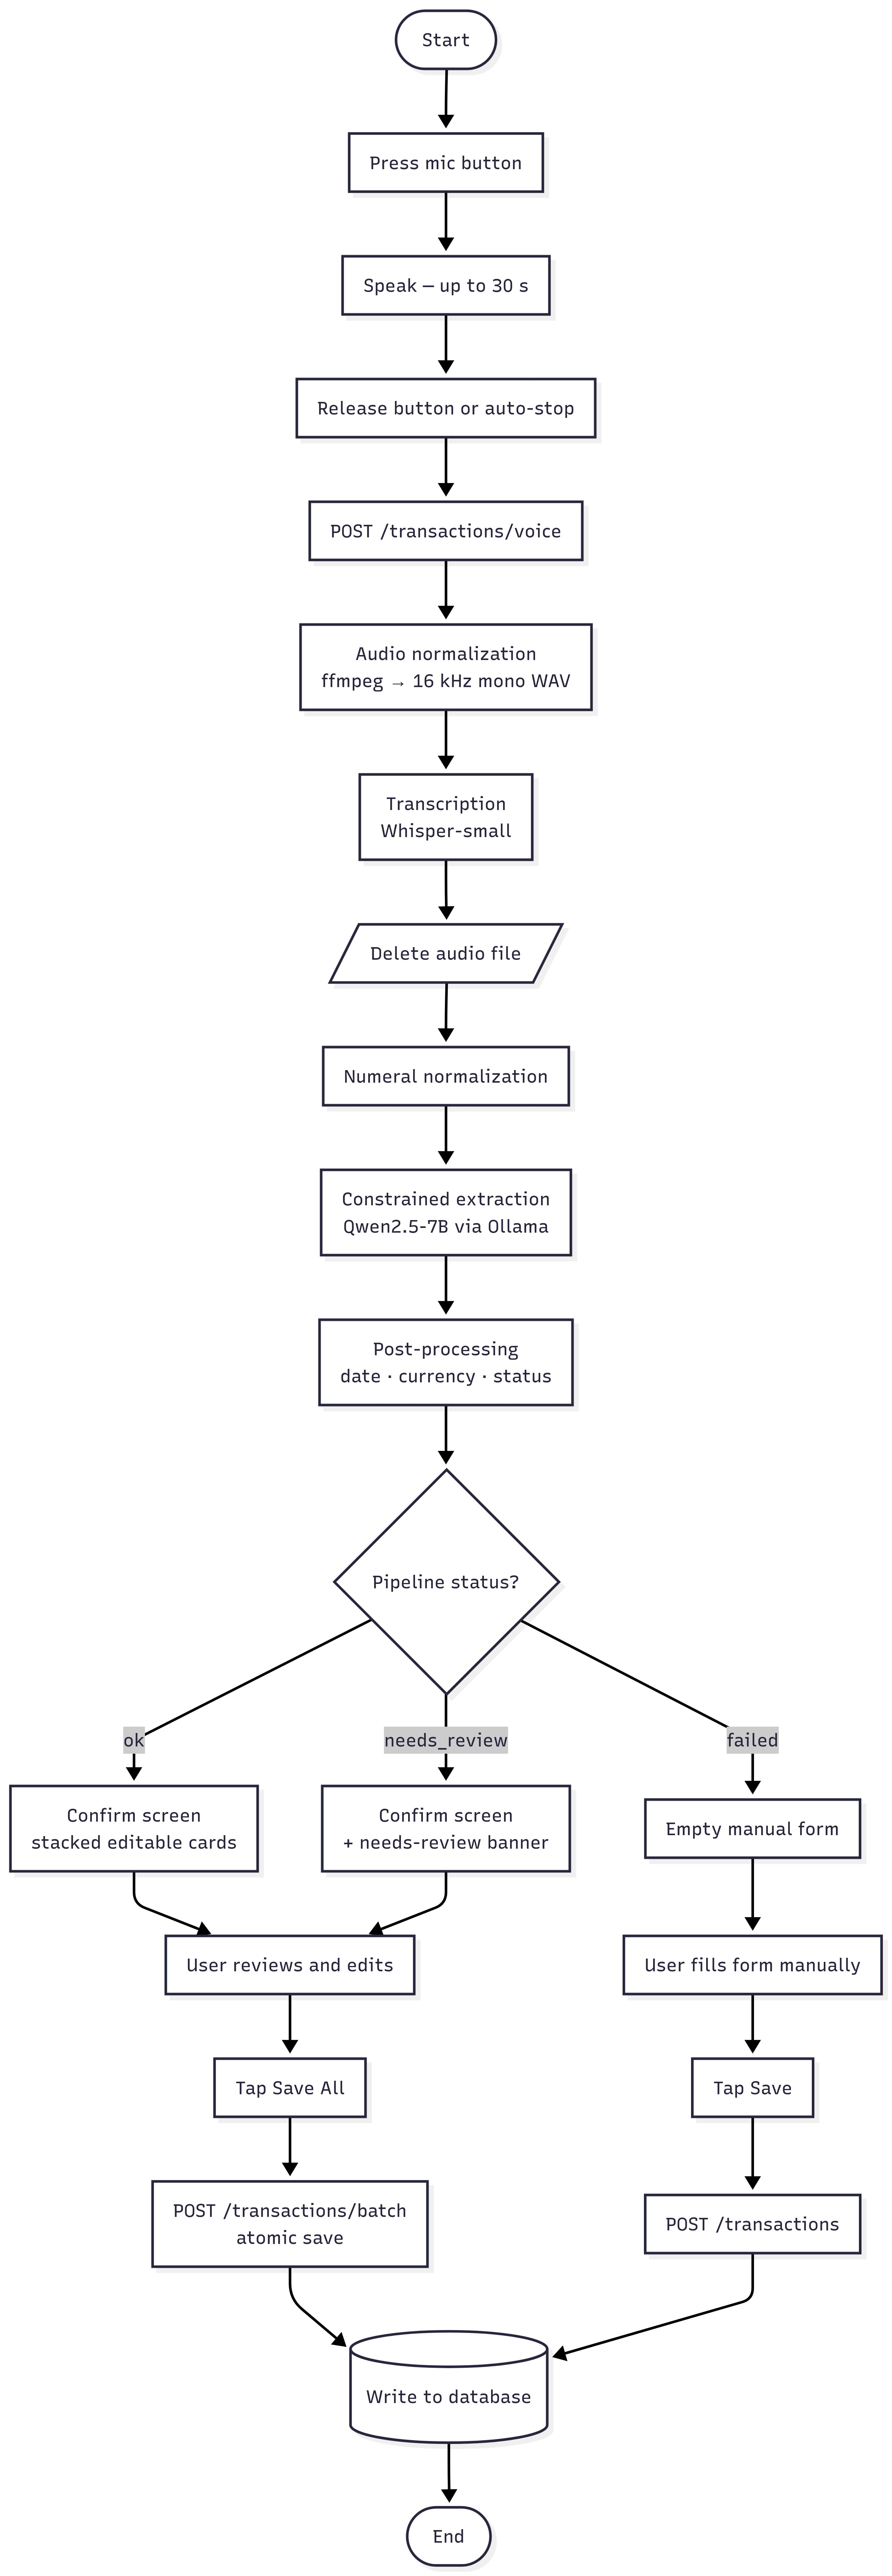
\includegraphics[height=0.85\textheight, keepaspectratio]{figures/activity_voice.jpg}



    \caption[Activity diagram: voice transaction]{Activity diagram for the voice
    transaction flow. After recording, the server transcribes, extracts, and
    post-processes; the resulting status branches the UI to a confirmation step
    (\texttt{ok}/\texttt{needs\_review}) or a manual form (\texttt{failed}). The
    save action is the only path that writes to the database.}
    \label{fig:activity-voice}
\end{figure}
\clearpage

\section{Class Diagram}

Figure~\ref{fig:class} shows the principal backend classes and their
relationships: the SQLAlchemy domain models (\texttt{User},
\texttt{Transaction}, \texttt{Category}), the Pydantic schemas that mediate the
API boundary, and the service layer (\texttt{STTService},
\texttt{extraction}, \texttt{postprocess}, \texttt{voice\_pipeline}). The service
layer is deliberately decoupled: \texttt{voice\_pipeline} orchestrates
\texttt{STTService} and the extraction/post-processing functions but depends on
them only through narrow interfaces, which is what allows the text-input mode to
reuse the same extraction core while bypassing speech-to-text.

\begin{figure}[H]
    \centering
    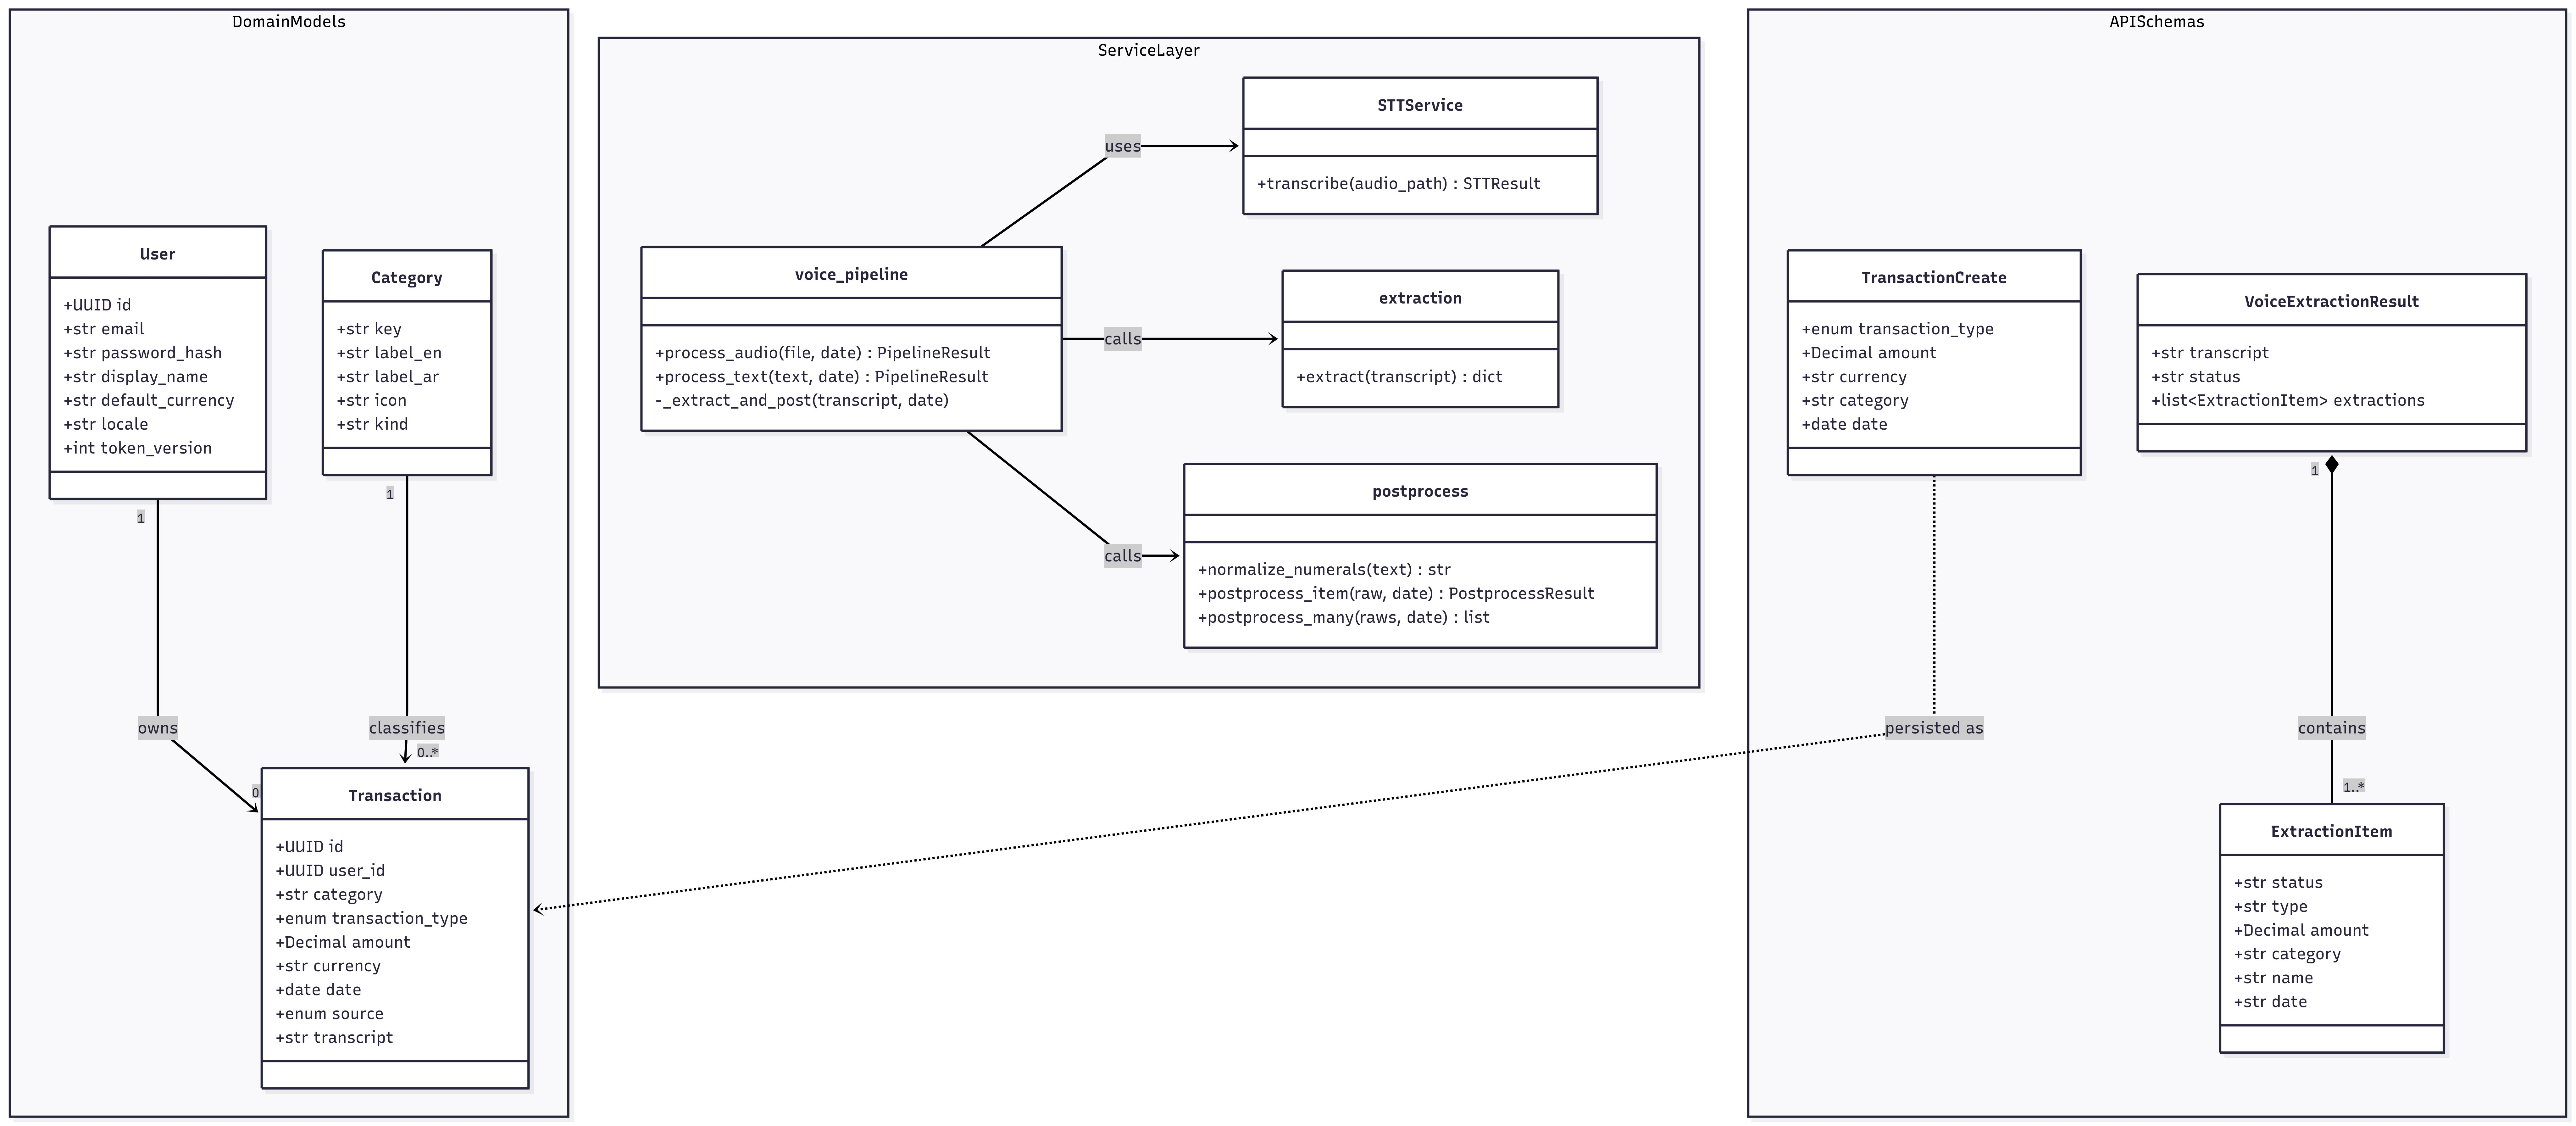
\includegraphics[width=\textwidth]{figures/class_diagram.jpg}
    \caption[Backend class diagram]{Backend class diagram. Domain models, API
    schemas, and the service layer. \texttt{voice\_pipeline} orchestrates the STT
    and extraction services through narrow interfaces; \texttt{process\_audio} and
    \texttt{process\_text} share a single \texttt{\_extract\_and\_post} core.}
    \label{fig:class}
\end{figure}

\section{Sequence Diagrams}

Two sequence diagrams capture the system's dynamic behavior. The first
(Figure~\ref{fig:seq-voice}) traces the voice transaction end-to-end, emphasizing
the two-step save: the voice endpoint returns an extraction but persists nothing;
a separate save call commits the user-confirmed records. The second
(Figure~\ref{fig:seq-auth}) traces authenticated request handling and the
transparent token-refresh interceptor on the client.

\begin{figure}[H]
    \centering
    \includegraphics[width=\textwidth]{figures/sequence_voice.jpg}
    \caption[Sequence diagram: voice to saved transaction]{Sequence diagram of the
    voice flow. The app uploads audio with the device date; the backend
    transcribes (Whisper), extracts (Ollama, constrained), post-processes, and
    returns the result. The user confirms, and only then does the app call the
    save endpoint, which inserts the records. The AI stage is stateless.}
    \label{fig:seq-voice}
\end{figure}

\begin{figure}[H]
    \centering
    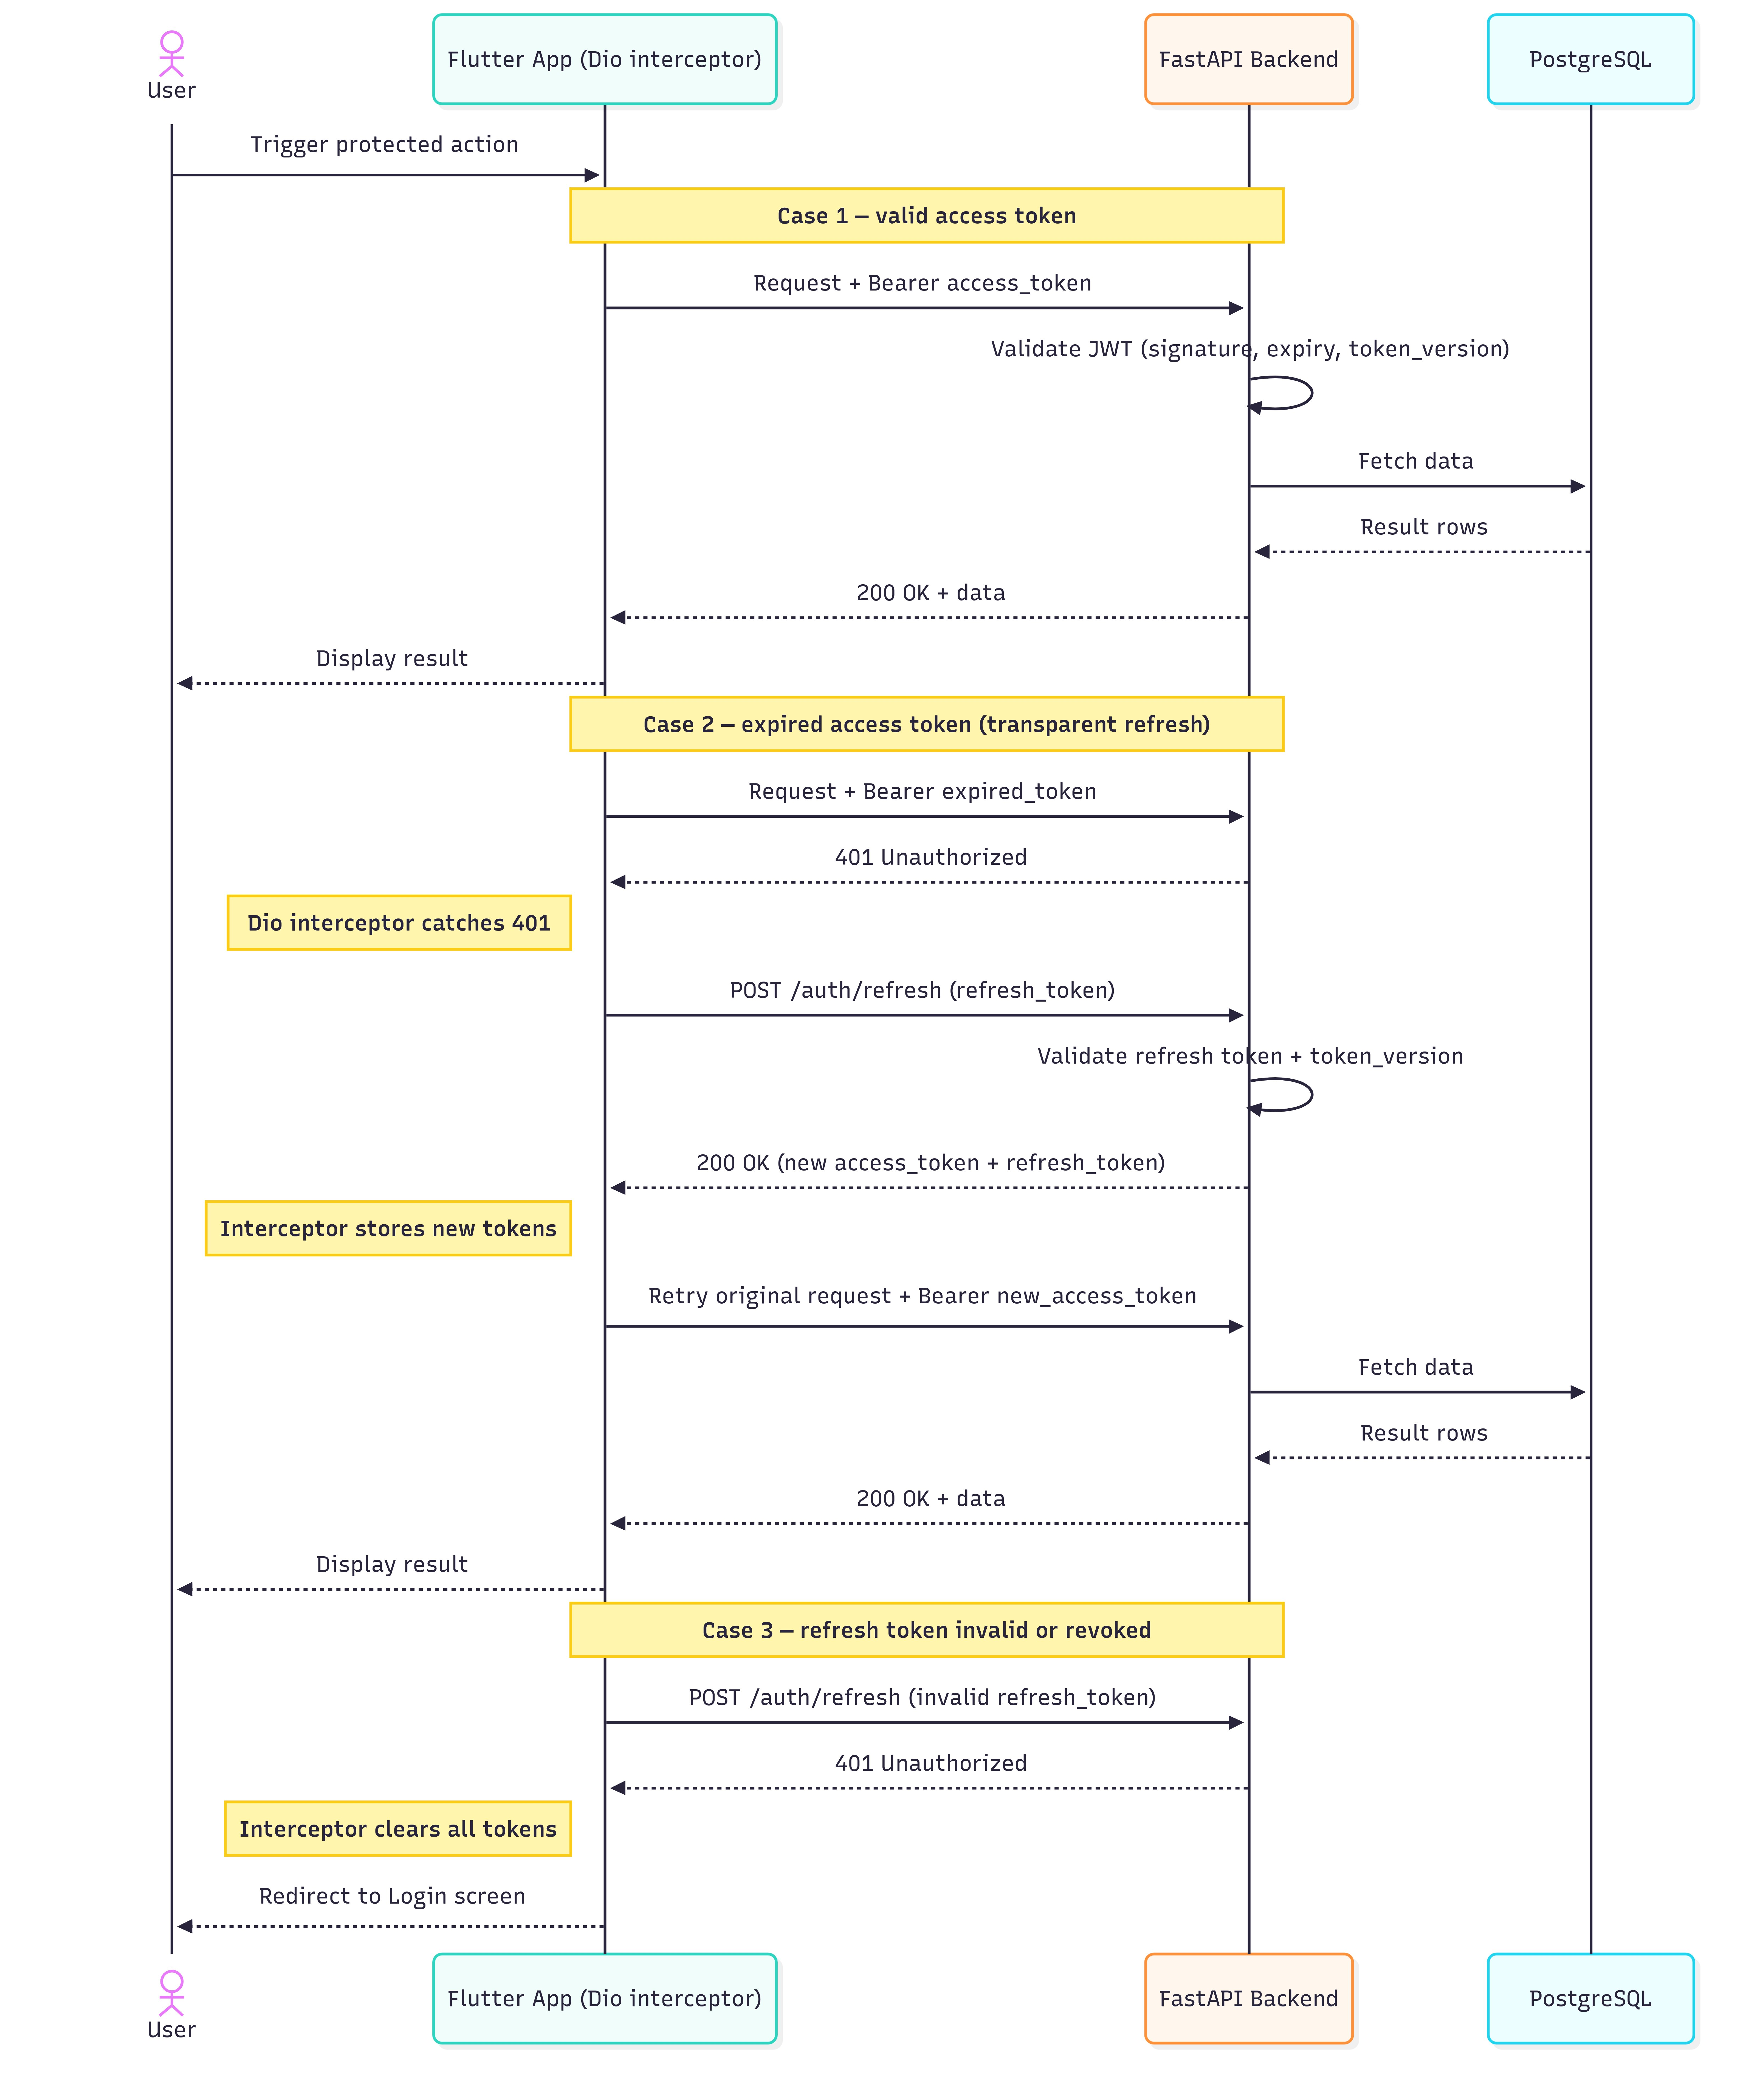
\includegraphics[width=0.9\textwidth]{figures/sequence_auth.jpg}
    \caption[Sequence diagram: authenticated request with token refresh]{Sequence
    diagram of authenticated request handling. On a 401 the client's interceptor
    transparently exchanges the refresh token for a new access token once, retries
    the request, and otherwise logs the user out.}
    \label{fig:seq-auth}
\end{figure}

\section{Use Case Scenarios}

The following scenarios specify the principal use cases in structured form. Each
lists the actor, preconditions, the main success scenario, and notable
alternative or exception flows.

\begin{table}[H]
\centering
\caption{Use case UC-01: Record a voice transaction.}
\label{tab:uc-voice}
\small
\renewcommand{\arraystretch}{1.3}
\begin{tabularx}{\textwidth}{>{\bfseries\raggedright\arraybackslash}p{3cm} X}
\toprule
Use case & UC-01 Record a voice transaction \\
\midrule
Actor & Authenticated user \\
Preconditions & User is logged in; microphone permission granted; backend healthy. \\
Main success & (1) User taps the mic and speaks. (2) User taps to stop. (3) App uploads audio with the device date and locale. (4) Backend transcribes, extracts, post-processes, returns a list of records with status \texttt{ok}. (5) App shows one editable card per record. (6) User confirms. (7) App saves all records atomically; they appear in the list. \\
Alternative & At step 4 the status is \texttt{needs\_review} (amount/type missing or low confidence): the affected cards are highlighted for the user to complete before saving. \\
Exception & The transcript is empty or no transaction is detected (\texttt{failed}): the app opens the manual entry form instead. The extraction service being unreachable yields an \texttt{EXTRACTION\_FAILED} error and the app offers manual entry. \\
\bottomrule
\end{tabularx}
\end{table}

\begin{table}[H]
\centering
\caption{Use case UC-02: Add a transaction by typing.}
\label{tab:uc-text}
\small
\renewcommand{\arraystretch}{1.3}
\begin{tabularx}{\textwidth}{>{\bfseries\raggedright\arraybackslash}p{3cm} X}
\toprule
Use case & UC-02 Add a transaction by typing \\
\midrule
Actor & Authenticated user \\
Preconditions & User is logged in; backend healthy. \\
Main success & (1) User types a sentence in Arabic, English, or a mix. (2) App calls the text-extraction endpoint (no speech stage). (3) Backend runs the same extraction and post-processing as voice. (4) App shows the same confirmation cards. (5) User confirms and saves. \\
Alternative & Multi-transaction sentence yields several cards saved atomically. \\
Exception & Empty/whitespace input is rejected with a validation error before any model call. \\
\bottomrule
\end{tabularx}
\end{table}

\begin{table}[H]
\centering
\caption{Use case UC-03: View the monthly dashboard.}
\label{tab:uc-dash}
\small
\renewcommand{\arraystretch}{1.3}
\begin{tabularx}{\textwidth}{>{\bfseries\raggedright\arraybackslash}p{3cm} X}
\toprule
Use case & UC-03 View the monthly dashboard \\
\midrule
Actor & Authenticated user \\
Preconditions & User is logged in; at least one transaction exists for the month. \\
Main success & (1) User opens the dashboard and selects a month. (2) App requests the monthly summary. (3) Backend aggregates the user's transactions for that month. (4) App shows total income, total expense, balance, and a category donut chart. \\
Alternative & No data for the selected month: an empty-state message is shown. \\
\bottomrule
\end{tabularx}
\end{table}

Together, these models---requirements, context, data flow, ER, use cases,
activities, classes, and sequences---fully specify what MiPay must do and how its
parts collaborate. The next chapter turns from analysis to construction,
describing how each model is realized in code.
